\chapter{Results and analysis}

In this chapter, the quantitative result data of the model selection process is presented and discussed along with diagrams that show a visual representation of the performance of the models.

\begin{figure}[h]
\centering
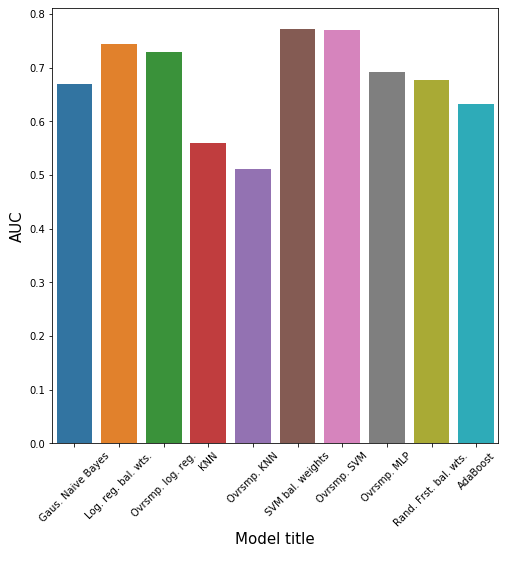
\includegraphics[width=0.9\linewidth]{results/fig/barplot.PNG}
\caption{Model AUC scores}
\label{fig:barplot}
\end{figure}

In Figure \ref{fig:barplot} the AUC scores of all the models averaged over 10-fold stratified cross validation are plotted. SVMs are a clear winner, being followed by Logistic Regression and MLP. The SVM with adjusted weights had an AUC score of 0.77 with a generalisation score of 0.56, Logistic Regression obtained 0.74 and 0.43 and the MLP got 0.69 and 0.57. The ROC curve for SVM is presented in Figure \ref{fig:rocsvm} and AUC scores and ROC curves for individual iterations can also be observed, as well as the standard deviation of the curve. The main curve is averaged over the 10 folds of the cross validation process. Similar ROC curves for Logistic Regression and MLP can be observed in Figure \ref{fig:roclog} and Figure \ref{fig:rocmlp}. 

\begin{figure}[h]
\centering
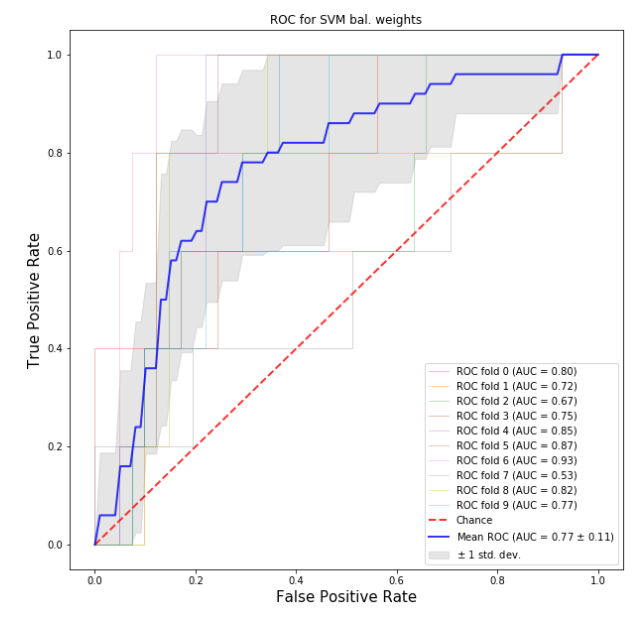
\includegraphics[width=0.7\linewidth]{results/fig/rocsvm.PNG}
\caption{ROC curve for SVM with balanced weights}
\label{fig:rocsvm}
\end{figure}

The Table \ref{tab:modelscores} contains all the metrics calculated for each of the models. When evaluating the performance of the models it is sometimes useful to look at several scores. For example, the MLP with over-sampling has a good AUC score which might indicate at first sight that the model performs well. However, the recall is quite low and that means the model is not good at identifying hits - what we are most interested in. That is also why a score such as the F1 score can be useful since it summarises both recall and precision (the percentage of hits that are correctly classified and the percentage of hit predictions that are correct). A graph with the F1 scores for the models plotted can be found in Figure \ref{fig:f1s}.

\begin{figure}[h]
    \centering
    \begin{minipage}{0.45\textwidth}
        \centering
        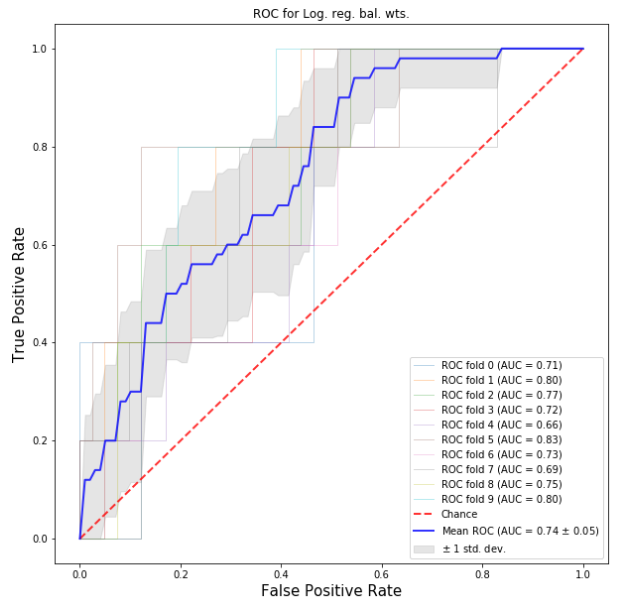
\includegraphics[width=0.9\textwidth]{results/fig/roclog.PNG} % first figure itself
        \caption{ROC curve for Log. Reg. with balanced weighs}
        \label{fig:roclog}
    \end{minipage}\hfill
    \begin{minipage}{0.45\textwidth}
        \centering
        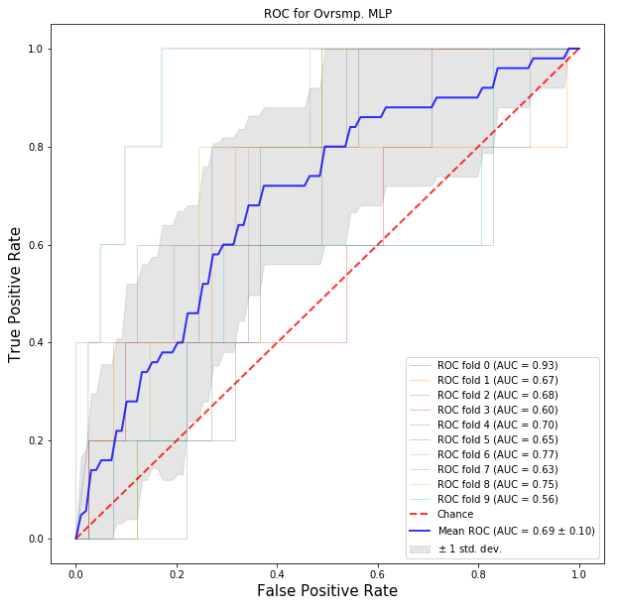
\includegraphics[width=0.9\textwidth]{results/fig/rocmlp.PNG} % second figure itself
        \caption{ROC curve for MLP with oversampling}
        \label{fig:rocmlp}
    \end{minipage}

\end{figure}

The results appear to be in line with some of the previous research where SVMs with an RBF kernel were the best performing model \cite{pham2016predicting}. This means that the data is most likely not linearly separable since the SVM uses something called a kernel trick to map the input into higher dimensional feature spaces. The good performance of some of the other models might be due to the fact that they assumes a linearly separable data space while that might not be the case or due to the particular advantages of the models.

However, due to the variation of experimentation methods in previous research in this area it is hard to accurately compare results. The data sets used are not the same, the features used are different and the way the data is labelled is different. Perhaps this is a further indication to the fact that this is still a field of ongoing research with a plethora of unexplored paths and opportunities. 

I believe the promising results in this project can be due to the smaller data set with recent songs used, the optimisation process and the way the data is labelled (by using the Spotify popularity metric and focusing only on the most popular songs).

\begin{table}[h]
% \begin{adjustbox}{max width=\textwidth}
\resizebox{\textwidth}{!}{%
\begin{tabular}{*{8}{|c}|}
\hline
\textbf{Model title}    & \textbf{Acc.} & \textbf{Spec.} & \textbf{Rec.} & \textbf{Prec.} & \textbf{F1} & \textbf{AUC} & \textbf{Gen. AUC}\\ \hline
Gaussian Naive Bayes    & 0.404             & 0.339                & 0.940                        & 0.149              & 0.257       & 0.670        & 0.421                           \\ \hline
Log. reg. bal. weights. & 0.639             & 0.634                & 0.680                        & 0.191              & 0.296       & 0.745        & 0.433                          \\ \hline
Over-sampling log. reg.  & 0.641             & 0.632                & 0.720                        & 0.194              & 0.304       & 0.730        & 0.454                           \\ \hline
KNN                     & 0.891             & 1.000                & 0.000                        & 0.000              & 0.000       & 0.560        & 0.685                           \\ \hline
Over-sampling KNN        & 0.739             & 0.802                & 0.220                        & 0.130              & 0.159       & 0.511        & 0.478                           \\ \hline
SVM bal. weights        & 0.628             & 0.607                & 0.800                        & 0.203              & 0.320       & {\ul 0.772}  & 0.566                          \\ \hline
Over-sampling SVM        & 0.743             & 0.749                & 0.700                        & 0.270              & {\ul 0.378} & 0.770        & 0.481                          \\ \hline
Over-sampling MLP        & 0.843             & 0.915                & 0.260                        & 0.248              & 0.250       & 0.693        & 0.572                          \\ \hline
Random Forest bal. wts. & 0.733             & 0.768                & 0.440                        & 0.190              & 0.262       & 0.676        & 0.382                           \\ \hline
AdaBoost                & 0.843             & 0.917                & 0.240                        & 0.235              & 0.234       & 0.633        & 0.486                           \\ \hline
\end{tabular}%
}
\caption{Table containing model scores}
\label{tab:modelscores}
\end{table}

